\section{Errore di previsione e bisogno di ricerca}
\label{sec:error}
\subsection{Come misuro l'errore}
Per capire se il modello ha imparato qualcosa di utile confronto le sue
previsioni con i target delle mappe escluse dall'allenamento. Per ogni
stato considero la differenza, in valore assoluto, fra costo di riferimento
e costo previsto; poi faccio la media di queste differenze.
Questa misura è l'\emph{errore assoluto medio}, abbreviato MAE.

Indico con $M$ il numero di esempi di verifica, con $s_i$ lo stato del
$i$-esimo esempio, con $y_i$ il suo target e con $\widehat h(s_i)$ la
previsione. La formula è
\[
 \operatorname{MAE}=\frac{1}{M}\sum_{i=1}^{M}\left|y_i-\widehat h(s_i)\right|.
\]
Un MAE minore indica previsioni mediamente più vicine ai target.

Per avere un confronto semplice considero anche un predittore che risponde
sempre con lo stesso numero: la media dei target di allenamento,
pari a $538{,}135$. Non è il metodo A: A cerca un percorso, mentre questa
previsione costante serve soltanto a valutare il modello.

Sui $120$ stati di verifica il modello ha MAE $49{,}391$, contro $184{,}684$
della costante: l'errore medio si riduce di circa il $73{,}26\%$.
Come controllo aggiuntivo, considero anche la radice della media degli
errori al quadrato, detta RMSE, che dà più peso agli errori grandi:
risulta $60{,}214$. Infine calcolo il \emph{bias}, cioè la media delle
differenze con segno fra previsione e target: è $0{,}175$.
Un bias vicino a zero non implica che le singole previsioni siano corrette:
le sovrastime possono compensare le sottostime.

\begin{figure}[!htbp]
\centering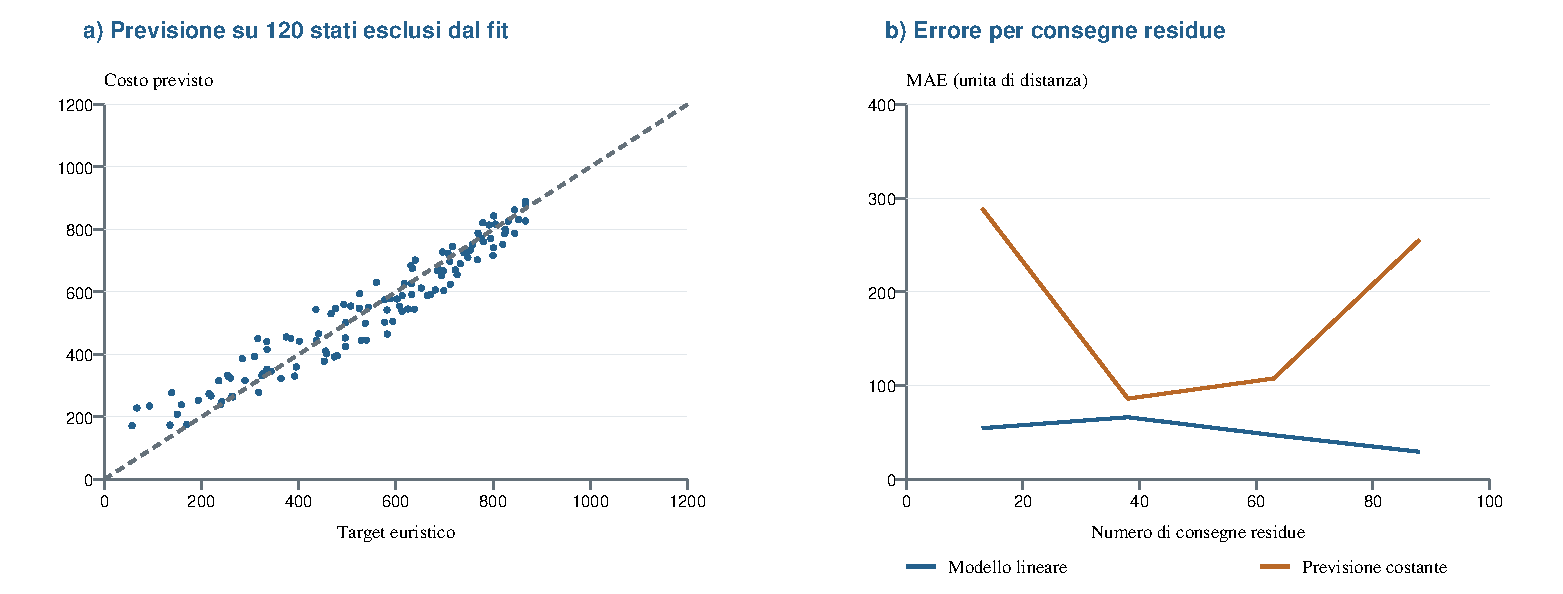
\includegraphics[width=\linewidth]{images/predictor.pdf}
\caption{A sinistra ogni punto confronta il target di uno stato con la
previsione: sulla diagonale i due valori coincidono. A destra confronto
l'errore medio del modello e della previsione costante in quattro intervalli
di consegne residue, ciascuno con 30 stati. Gli stati provengono da sole
tre mappe e non sono osservazioni indipendenti.}\label{fig:predictor}
\end{figure}

L'accuratezza cambia con il numero di consegne rimaste. Negli intervalli
$1$--$25$, $26$--$50$, $51$--$75$ e $76$--$100$, i MAE sono rispettivamente
$54{,}632$, $66{,}334$, $47{,}150$ e $29{,}448$.
Anche fra le tre mappe l'errore medio varia: $37{,}237$, $51{,}159$ e
$59{,}777$. La sola media globale nasconderebbe queste differenze.
Poiché i target grandi sono approssimati, questi valori misurano la distanza
dall'insegnante, non l'errore esatto rispetto al giro ottimo.

\subsection{Errore e utilità di continuare a cercare}
Posso anche chiedermi di quanto una singola previsione cambi dopo aver
approfondito la ricerca. Chiamo questa differenza \emph{residuo}.
Indico con $h_{\mathrm{rif}}(s)$ il costo rimanente ottenuto dal riferimento
e con $r(s)$ il residuo:
\[
 r(s)=h_{\mathrm{rif}}(s)-\widehat h(s).
\]
Un residuo positivo significa che il modello prevedeva un costo troppo
basso; uno negativo significa che lo prevedeva troppo alto, rispetto
al riferimento. La stessa differenza si ottiene confrontando costi totali,
perché la distanza già percorsa è uguale nei due valori e si cancella.

Conoscere il residuo richiede la ricerca aggiuntiva del riferimento:
non è un'informazione disponibile in anticipo al regolatore.
Inoltre, un ramo con un grande errore di previsione può comunque portare
a un giro peggiore degli altri. L'entità dell'errore e il beneficio di
esplorare quel ramo sono quindi due quantità diverse.
Il caso piccolo della Sezione~8 rende concreta questa distinzione.

Non alleno un secondo modello per prevedere l'errore. Il regolatore usa
la stagnazione come segnale per cambiare candidato e le prove verificano
se questa scelta migliora i giri trovati. Non dimostro una relazione
statistica fra stagnazione, residuo e miglioramento futuro: è un limite
della proposta.
